\begin{enumerate}
	\item  Let us consider $A:= \begin{bmatrix}a_{11}&a_{12}\\a_{21}&a_{22}\end{bmatrix} $ with $a_{12} = a_{21}$ and first analye the property for being $A$ being positive definite. We see
	\begin{align*}
		x^TAx=a_{11}x_1^2+a_{12}x_1x_2+a_{12}x_2x_1+a_{22}x_2^2
		=a_{11}x_1^2+2a_{12}x_1x_2+a_{22}x_2^2
		\stackrel{!}{>} 0\ \ \forall x=(x_1,x_2)^\top\neq (0,0)^\top.
		\end{align*}
	\underline{Example:}
	\begin{align*}
		A=\begin{bmatrix}2&1\\1&2\end{bmatrix},~ x^TAx &=\overbrace{2x_1^2}^{\textcolor{blue}{x_1^2+x_1^2}}+2x_1x_2+2x_2^2\\
		&=x_1^2+x_2^2+\underbrace{(x_1+x_2)^2}_{\geq0}\\
		&\geq x_1^2+x_2^2\\
		&>0~~~~~~~~~ \forall\begin{pmatrix}x_1\\x_2\end{pmatrix}\neq\begin{pmatrix}0\\0\end{pmatrix}
		\end{align*}
	\item  Consider
	$\{Ax:\|{x}\|_2 =1\}$ with $\ A=\begin{bmatrix}2&1\\1&2\end{bmatrix}$. Also recall from the lecture that $\left(3, \begin{bmatrix}1\\1\end{bmatrix}\right), \left(1, \begin{bmatrix}1\\-1\end{bmatrix}\right)$ are eigenpairs (see later).
	\begin{center}
		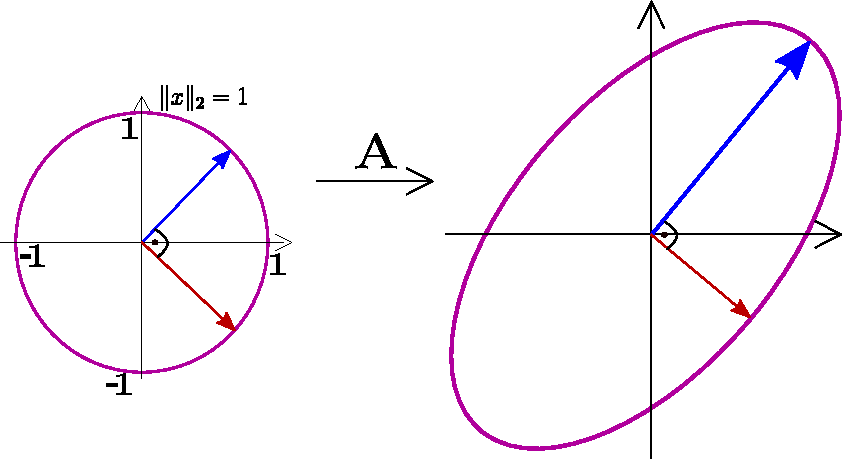
\includegraphics[width=0.6\textwidth]{spdMatrix.pdf}
	\end{center}
	~\\Further general note:
	\begin{center}
		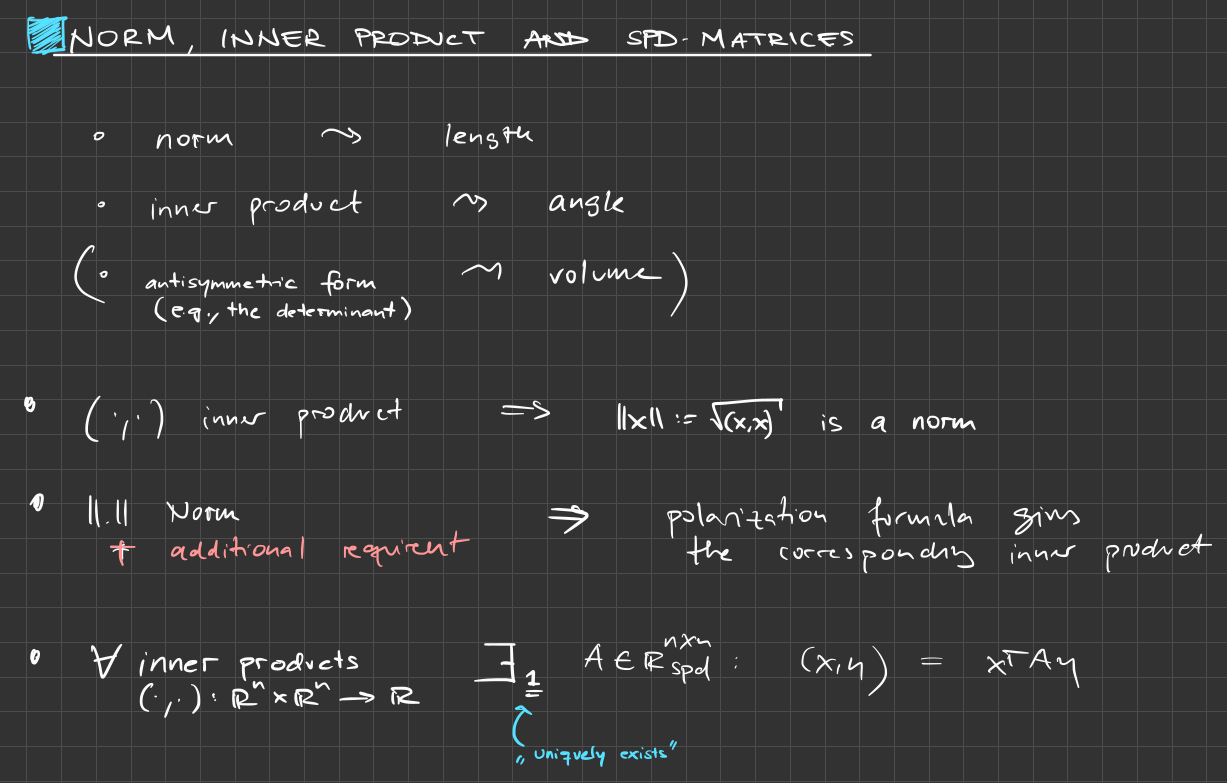
\includegraphics[width=0.99\linewidth]{ex-spdMatsAndNorms}
	\end{center}
	
\end{enumerate}